\documentclass[12pt,x11names,a4paper]{article}
\input{preamble}


\newgeometry{margin=2cm}

\pagestyle{fancy}
\fancyhf{}

\rhead{Nørre Gymnasium\\1.m
}
\cfoot{Side \thepage \hspace{1pt} af \pageref{LastPage}}

%Husk at rette modul og dato!
\lhead{Aflevering 5\\ Matematik B
}
\chead{8. marts
}

\begin{document}

%\includepdf[pages=-]{Forsider/aarsprove_1v.pdf}
\savegeometry{art}

\begin{titlepage}
\newgeometry{margin=0pt}

\begin{minipage}{0.27\textwidth}

\begin{tikzpicture}[overlay]
\fill[top color = NorregGroen!40, bottom color = NorregGroen] (6,10) rectangle (-10,-30);
\end{tikzpicture}
\end{minipage}
\begin{minipage}{0.73\textwidth}
\begin{center}
\phantom{h} \vspace{1cm}\\
\hspace{4cm}
\includegraphics[scale = 1]{Billeder/Norreg.png} \\
\phantom{h} \vspace{5cm}\\
\rule{0.7\textwidth}{0.3mm}\\
\phantom{h}\\
{\fontsize{50}{60}\selectfont Aflevering 4}\\
\phantom{h}\\
\rule{0.7\textwidth}{0.3mm}\\
\Large 2024\\
\Large 1.m Ma

\end{center}
\end{minipage}
\end{titlepage}
\loadgeometry{art}

%Udfyld afsnit herunder og lav til egen Latex-fil

%Kopier følgende til overskrift:

%\begin{center}
%\Huge
%Aflevering 1
%\end{center}
%\section*{Opgave 1}
%\stepcounter{section}
\begin{center}
%Opgavesætter er delt i to dele:\\
%Delprøve 1 kun med den centralt udmeldte formelsamling.\\
%Delprøve 2 med alle hjælpemidler.
\end{center}

\section*{Krav til formidling af din besvarelse}

Ved bedømmelse af helhedsindtrykket af besvarelsen af de enkelte opgaver lægges særlig vægt på følgende fire punkter:
\begin{itemize}
\item[$\cdot$] \textbf{Redegørelse og dokumentation for metode} \\
Besvarelsen skal indeholde en redegørelse for den anvendte løsningsstragegi med dokumentation i form af et passende antal mellemregninger \textit{eller} matematiske forklaringer på metoden, når et matematisk værktøjsprogram anvendes.
\item[$\cdot$] \textbf{Figurer, grafer og andre illustrationer} \\
Besvarelsen skal indeholde hensigtsmæssig brug af figurer, grafer og andre illustrationer, og der skal være tydelige henvisninger til brug af disse i den forklarende tekst.
\item[$\cdot$] \textbf{Notation og layout}\\
Besvarelsen skal i overensstemmelse med god matematisk skik opstilles med hensigtsmæssig brug af symbolsprog, og med en redegørelse for den matematiske notation, der indføres og anvendes, og som ikke kan henføres stil standardviden.
\item[$\cdot$] \textbf{Formidling og forklaring}\\
Besvarelsen af rene matematikopgaver skal indeholde en angivelse af givne oplysninger og korte forklaringer knyttet til den anvendte løsningsstrategi beskrevet med brug af almindelig matematisk notation. 

Besvarelsen af opgaver, der omhandler matematiske modeller, skal indeholde en kort præsentation af modellens kontekst, herunder betydning af modellens parametre. De enkelte delspørgsmål skal afsluttes med en præcis konklusion præsenteret i et klart sprog i relation til konteksten.
\end{itemize}

\newpage

\begin{center}
	\LARGE Uden hjælpemidler
\end{center}
\begin{opgavetekst}{Opgave 1}
	En stykvist defineret funktion er givet ved
	\begin{align*}
		f(x) = \begin{cases}
			-2x + 1, &\textnormal{ hvis } x \geq 2,\\
			x^2, &\textnormal{ hvis } x < 2.
		\end{cases}
	\end{align*}
\end{opgavetekst}
\begin{delopgave}{}{1}
	Bestem $f(-3)$
\end{delopgave}
\begin{delopgave}{}{2}
	Løs ligningen $f(x) = -5$.
\end{delopgave}
%%%%%%%%%%%%%%%%%%%%%%%%%%%%%%%%%%%%%%%%%%%%%%%%%%%%%%%%%%%%%%%%%%%%%%%%%%%%%%%%%%%%%%%%%%%%%%%%
%%%%%%%%%%%%%%%%%%%%%%%%%%%%%%%%%%%%%%%%%%%%%%%%%%%%%%%%%%%%%%%%%%%%%%%%%%%%%%%%%%%%%%%%%%%%%%%%
%%%%%%%%%%%%%%%%%%%%%%%%%%%%%%%%%%%%%%%%%%%%%%%%%%%%%%%%%%%%%%%%%%%%%%%%%%%%%%%%%%%%%%%%%%%%%%%%
%%%%%%%%%%%%%%%%%%%%%%%%%%%%%%%%%%%%%%%%%%%%%%%%%%%%%%%%%%%%%%%%%%%%%%%%%%%%%%%%%%%%%%%%%%%%%%%%
%%%%%%%%%%%%%%%%%%%%%%%%%%%%%%%%%%%%%%%%%%%%%%%%%%%%%%%%%%%%%%%%%%%%%%%%%%%%%%%%%%%%%%%%%%%%%%%%
%%%%%%%%%%%%%%%%%%%%%%%%%%%%%%%%%%%%%%%%%%%%%%%%%%%%%%%%%%%%%%%%%%%%%%%%%%%%%%%%%%%%%%%%%%%%%%%%
%%%%%%%%%%%%%%%%%%%%%%%%%%%%%%%%%%%%%%%%%%%%%%%%%%%%%%%%%%%%%%%%%%%%%%%%%%%%%%%%%%%%%%%%%%%%%%%%
%%%%%%%%%%%%%%%%%%%%%%%%%%%%%%%%%%%%%%%%%%%%%%%%%%%%%%%%%%%%%%%%%%%%%%%%%%%%%%%%%%%%%%%%%%%%%%%%
\begin{opgavetekst}{Opgave 2}
	To funktioner $f$ og $g$ er givet ved henholdsvis
	\begin{align*}
		f(x) = \sqrt{x}
	\end{align*}
	og
	\begin{align*}
		g(x) = x^2-2x+4.
	\end{align*}
\end{opgavetekst}
\begin{delopgave}{}{1}
	Bestem forskriften for den sammensatte funktion
	\begin{align*}
		h(x) = f(g(x))
	\end{align*}
\end{delopgave}
\begin{delopgave}{}{2}
	Bestem $f(g(2))$
\end{delopgave}
%%%%%%%%%%%%%%%%%%%%%%%%%%%%%%%%%%%%%%%%%%%%%%%%%%%%%%%%%%%%%%%%%%%%%%%%%%%%%%%%%%%%%%%%%%%%%%%%
%%%%%%%%%%%%%%%%%%%%%%%%%%%%%%%%%%%%%%%%%%%%%%%%%%%%%%%%%%%%%%%%%%%%%%%%%%%%%%%%%%%%%%%%%%%%%%%%
%%%%%%%%%%%%%%%%%%%%%%%%%%%%%%%%%%%%%%%%%%%%%%%%%%%%%%%%%%%%%%%%%%%%%%%%%%%%%%%%%%%%%%%%%%%%%%%%
%%%%%%%%%%%%%%%%%%%%%%%%%%%%%%%%%%%%%%%%%%%%%%%%%%%%%%%%%%%%%%%%%%%%%%%%%%%%%%%%%%%%%%%%%%%%%%%%
%%%%%%%%%%%%%%%%%%%%%%%%%%%%%%%%%%%%%%%%%%%%%%%%%%%%%%%%%%%%%%%%%%%%%%%%%%%%%%%%%%%%%%%%%%%%%%%%
%%%%%%%%%%%%%%%%%%%%%%%%%%%%%%%%%%%%%%%%%%%%%%%%%%%%%%%%%%%%%%%%%%%%%%%%%%%%%%%%%%%%%%%%%%%%%%%%
%%%%%%%%%%%%%%%%%%%%%%%%%%%%%%%%%%%%%%%%%%%%%%%%%%%%%%%%%%%%%%%%%%%%%%%%%%%%%%%%%%%%%%%%%%%%%%%%
%%%%%%%%%%%%%%%%%%%%%%%%%%%%%%%%%%%%%%%%%%%%%%%%%%%%%%%%%%%%%%%%%%%%%%%%%%%%%%%%%%%%%%%%%%%%%%%%
\newpage
\begin{opgavetekst}{Opgave 3}
	For en bestemt bil gælder der, at den forbrugte mængde brændstof $x$ (i L) er ligefrem proportional med den kørte afstand $y$ (i km). Proportionalitetskonstanten er 18.
\end{opgavetekst}
\begin{delopgave}{}{1}
	Opskriv en sammenhæng mellem $x$ og $y$. 
\end{delopgave}
\begin{delopgave}{}{2}
	Bestem hvor langt bilen kan køre på 3 liter brændstof
\end{delopgave}
\begin{delopgave}{}{3}
	Afgør, hvor meget brændstof bilen har forbrændt på 162 km. 
\end{delopgave}
%%%%%%%%%%%%%%%%%%%%%%%%%%%%%%%%%%%%%%%%%%%%%%%%%%%%%%%%%%%%%%%%%%%%%%%%%%%%%%%%%%%%%%%%%%%%%%%%
%%%%%%%%%%%%%%%%%%%%%%%%%%%%%%%%%%%%%%%%%%%%%%%%%%%%%%%%%%%%%%%%%%%%%%%%%%%%%%%%%%%%%%%%%%%%%%%%
%%%%%%%%%%%%%%%%%%%%%%%%%%%%%%%%%%%%%%%%%%%%%%%%%%%%%%%%%%%%%%%%%%%%%%%%%%%%%%%%%%%%%%%%%%%%%%%%
%%%%%%%%%%%%%%%%%%%%%%%%%%%%%%%%%%%%%%%%%%%%%%%%%%%%%%%%%%%%%%%%%%%%%%%%%%%%%%%%%%%%%%%%%%%%%%%%
%%%%%%%%%%%%%%%%%%%%%%%%%%%%%%%%%%%%%%%%%%%%%%%%%%%%%%%%%%%%%%%%%%%%%%%%%%%%%%%%%%%%%%%%%%%%%%%%
%%%%%%%%%%%%%%%%%%%%%%%%%%%%%%%%%%%%%%%%%%%%%%%%%%%%%%%%%%%%%%%%%%%%%%%%%%%%%%%%%%%%%%%%%%%%%%%%
%%%%%%%%%%%%%%%%%%%%%%%%%%%%%%%%%%%%%%%%%%%%%%%%%%%%%%%%%%%%%%%%%%%%%%%%%%%%%%%%%%%%%%%%%%%%%%%%
%%%%%%%%%%%%%%%%%%%%%%%%%%%%%%%%%%%%%%%%%%%%%%%%%%%%%%%%%%%%%%%%%%%%%%%%%%%%%%%%%%%%%%%%%%%%%%%%
\newpage
\begin{opgavetekst}{Opgave 4}
	Afgør, om følgende sammenhænge er ligefrem eller omvendt proportionale.
\end{opgavetekst}
\begin{delopgave}{}{1}
	\begin{align*}
		&a) \ y = 4x   &    &b) \  y\cdot x = 12   \\
		&c) \ \frac{y}{x} = -0.2  &    &d) \ y = \frac{4.15}{x}    \\
	\end{align*}
\end{delopgave}
%%%%%%%%%%%%%%%%%%%%%%%%%%%%%%%%%%%%%%%%%%%%%%%%%%%%%%%%%%%%%%%%%%%%%%%%%%%%%%%%%%%%%%%%%%%%%%%%
%%%%%%%%%%%%%%%%%%%%%%%%%%%%%%%%%%%%%%%%%%%%%%%%%%%%%%%%%%%%%%%%%%%%%%%%%%%%%%%%%%%%%%%%%%%%%%%%
%%%%%%%%%%%%%%%%%%%%%%%%%%%%%%%%%%%%%%%%%%%%%%%%%%%%%%%%%%%%%%%%%%%%%%%%%%%%%%%%%%%%%%%%%%%%%%%%
%%%%%%%%%%%%%%%%%%%%%%%%%%%%%%%%%%%%%%%%%%%%%%%%%%%%%%%%%%%%%%%%%%%%%%%%%%%%%%%%%%%%%%%%%%%%%%%%
%%%%%%%%%%%%%%%%%%%%%%%%%%%%%%%%%%%%%%%%%%%%%%%%%%%%%%%%%%%%%%%%%%%%%%%%%%%%%%%%%%%%%%%%%%%%%%%%
%%%%%%%%%%%%%%%%%%%%%%%%%%%%%%%%%%%%%%%%%%%%%%%%%%%%%%%%%%%%%%%%%%%%%%%%%%%%%%%%%%%%%%%%%%%%%%%%
%%%%%%%%%%%%%%%%%%%%%%%%%%%%%%%%%%%%%%%%%%%%%%%%%%%%%%%%%%%%%%%%%%%%%%%%%%%%%%%%%%%%%%%%%%%%%%%%
%%%%%%%%%%%%%%%%%%%%%%%%%%%%%%%%%%%%%%%%%%%%%%%%%%%%%%%%%%%%%%%%%%%%%%%%%%%%%%%%%%%%%%%%%%%%%%%%

\newpage

\begin{center}
	\LARGE Med hjælpemidler
\end{center}



\begin{opgavetekst}{Opgave 5}
	\begin{center}
		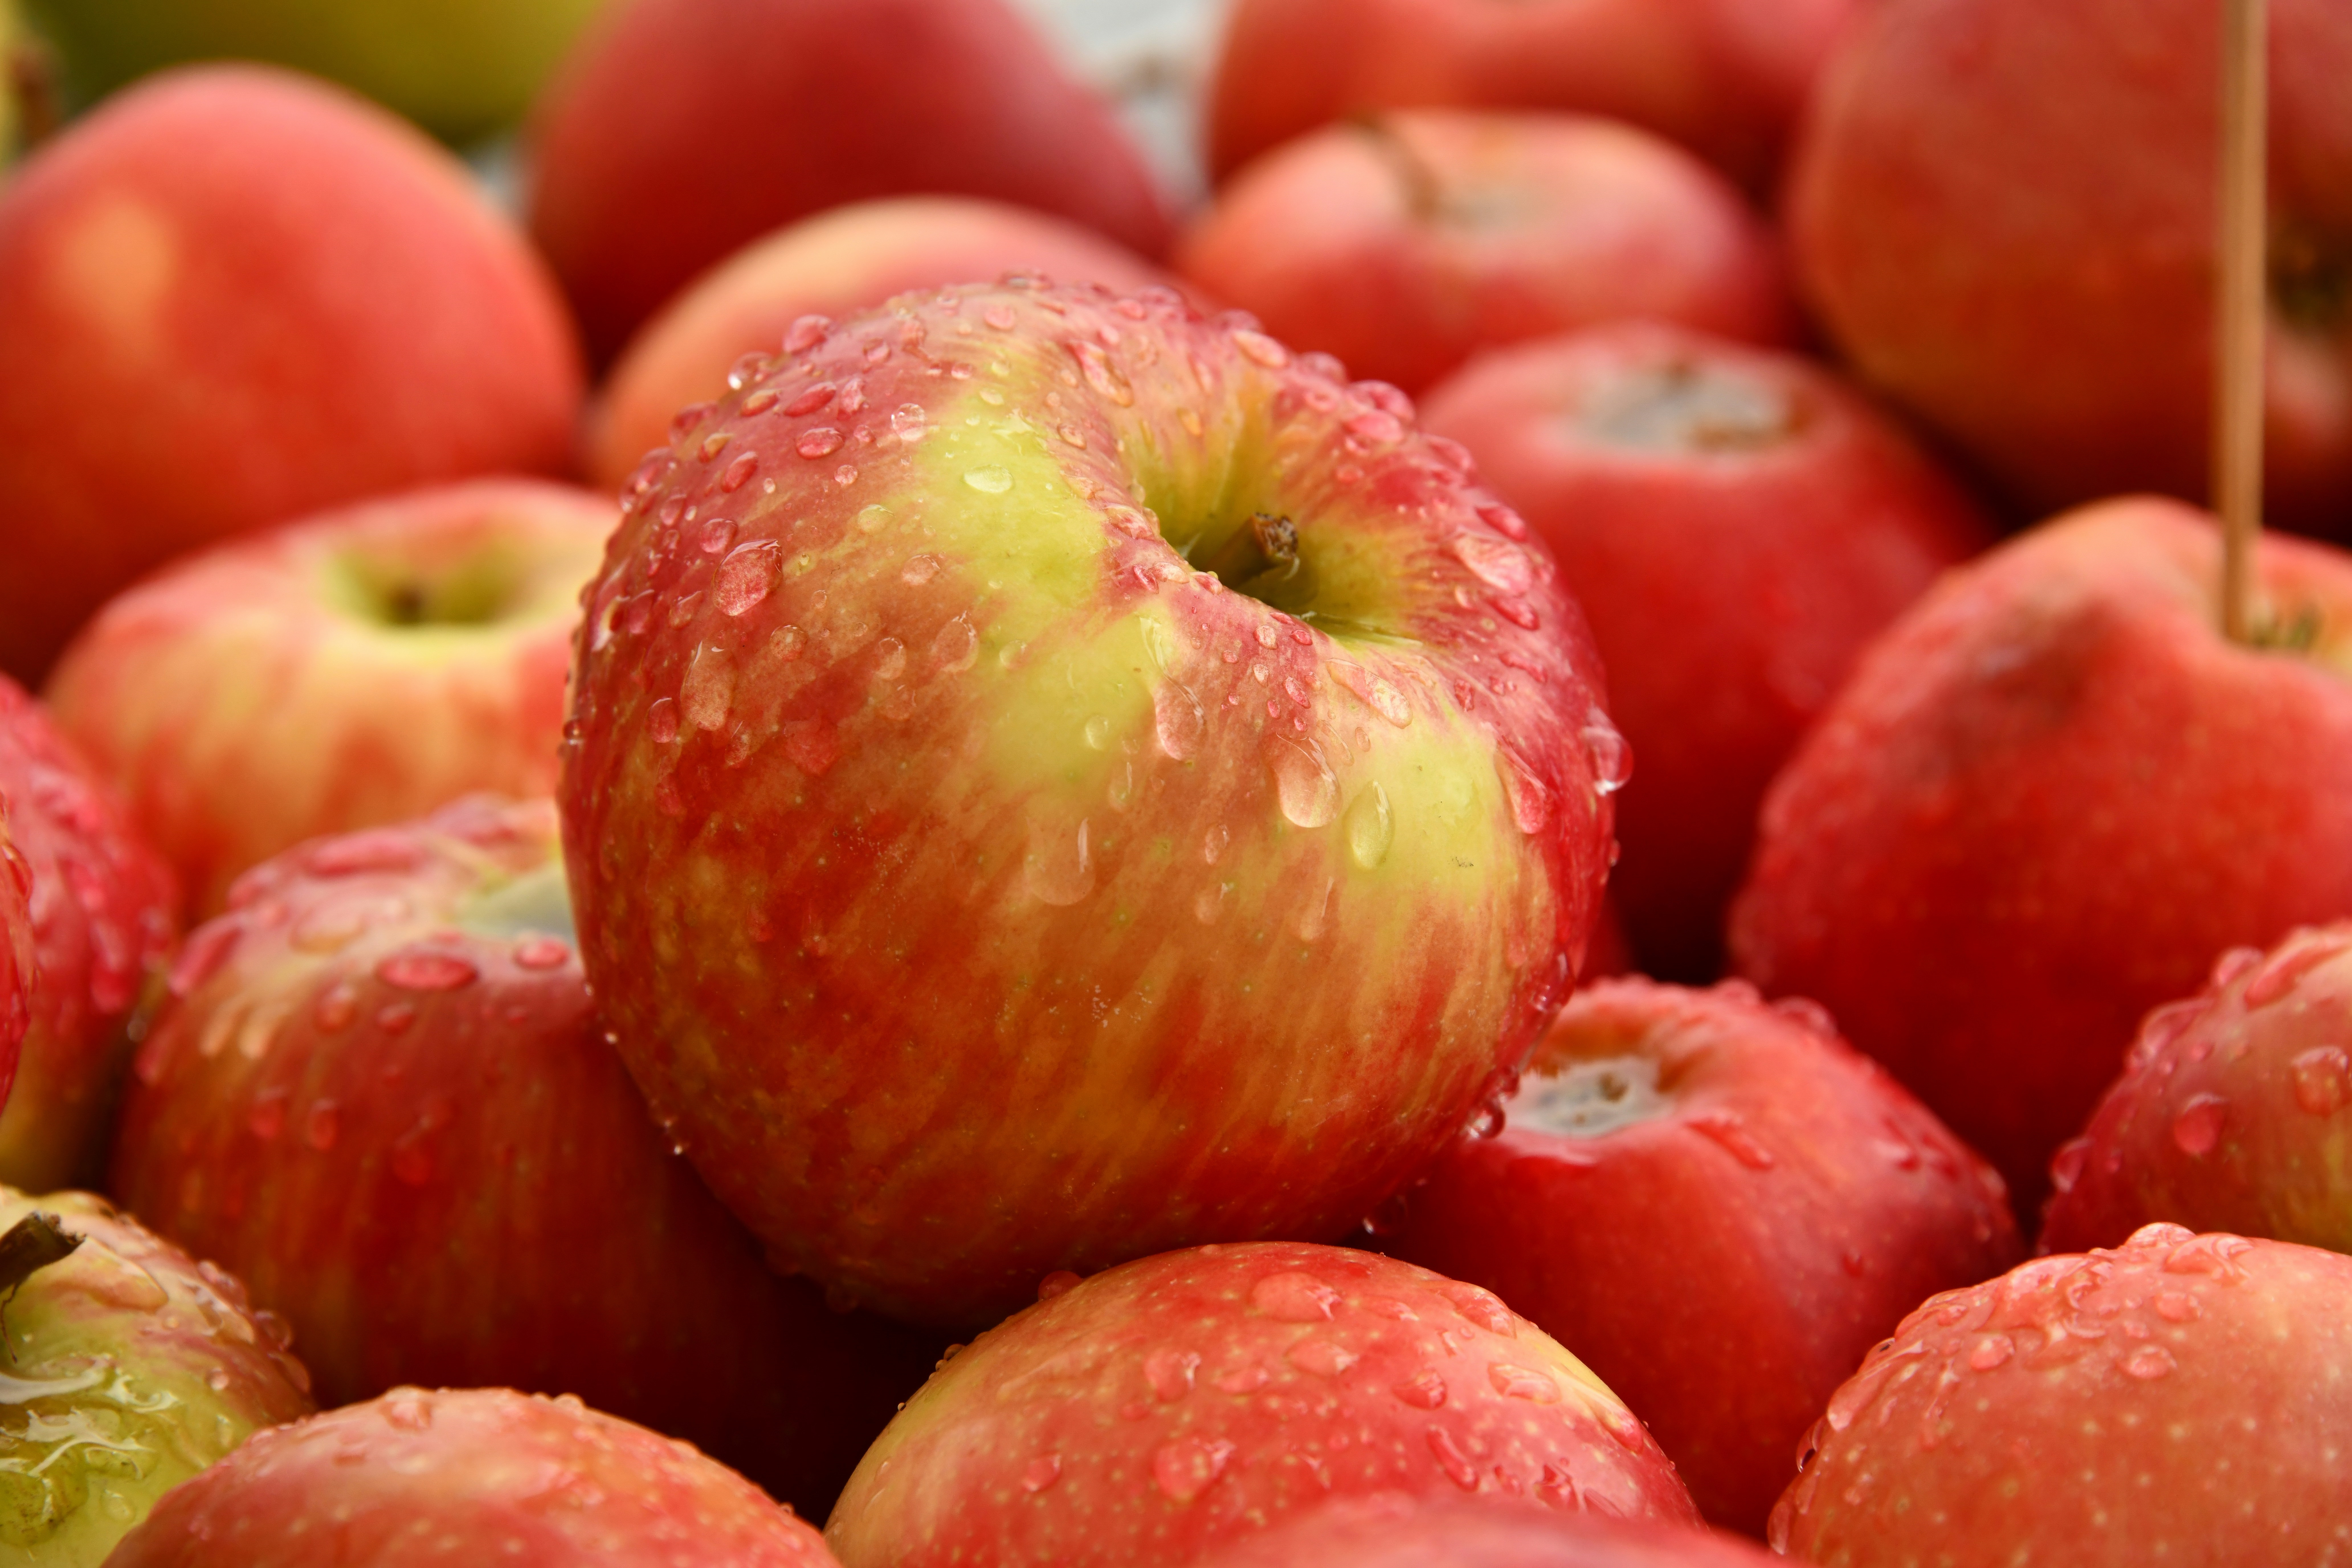
\includegraphics[width = 0.6\textwidth]{Billeder/apples}
	\end{center}	
	En dreng har målt højden og vægten af en række æbler. Resultatet af hans målinger kan 
	findes i \href{https://github.com/ChristianJLex/TeachingNotes/raw/master/2023-2024/Data og lign/aeble.xlsx}{\color{blue!60} dette datasæt.} Han ved ikke, om sammenhængen mellem vægten er en potenssammenhæng, en lineær sammenhæng eller en eksponentiel sammenhæng.
\end{opgavetekst}
\begin{delopgave}{}{1}
	Lav regressioner på datasættet og anvend residualanalyse til at afgøre hvilken model, der 
	bedst beskriver sammenhængen mellem æblernes højde og vægt.
\end{delopgave}	
\begin{delopgave}{}{2}
	Brug din valgte model til at afgøre, hvor højt et æble der vejer 300 gram er.
\end{delopgave}
\begin{delopgave}{}{3}
	Brug din valgte model til at afgøre, hvad et æble der er 4 cm vil veje.
\end{delopgave}
%%%%%%%%%%%%%%%%%%%%%%%%%%%%%%%%%%%%%%%%%%%%%%%%%%%%%%%%%%%%%%%%%%%%%%%%%%%%%%%%%%%%%%%%%%%%%%%%
%%%%%%%%%%%%%%%%%%%%%%%%%%%%%%%%%%%%%%%%%%%%%%%%%%%%%%%%%%%%%%%%%%%%%%%%%%%%%%%%%%%%%%%%%%%%%%%%
%%%%%%%%%%%%%%%%%%%%%%%%%%%%%%%%%%%%%%%%%%%%%%%%%%%%%%%%%%%%%%%%%%%%%%%%%%%%%%%%%%%%%%%%%%%%%%%%
%%%%%%%%%%%%%%%%%%%%%%%%%%%%%%%%%%%%%%%%%%%%%%%%%%%%%%%%%%%%%%%%%%%%%%%%%%%%%%%%%%%%%%%%%%%%%%%%
%%%%%%%%%%%%%%%%%%%%%%%%%%%%%%%%%%%%%%%%%%%%%%%%%%%%%%%%%%%%%%%%%%%%%%%%%%%%%%%%%%%%%%%%%%%%%%%%
%%%%%%%%%%%%%%%%%%%%%%%%%%%%%%%%%%%%%%%%%%%%%%%%%%%%%%%%%%%%%%%%%%%%%%%%%%%%%%%%%%%%%%%%%%%%%%%%
%%%%%%%%%%%%%%%%%%%%%%%%%%%%%%%%%%%%%%%%%%%%%%%%%%%%%%%%%%%%%%%%%%%%%%%%%%%%%%%%%%%%%%%%%%%%%%%%
%%%%%%%%%%%%%%%%%%%%%%%%%%%%%%%%%%%%%%%%%%%%%%%%%%%%%%%%%%%%%%%%%%%%%%%%%%%%%%%%%%%%%%%%%%%%%%%%
\begin{opgavetekst}{Opgave 6}
	Prisen for at rejse med taxafirmaet taxA kan beskrives ved funktionen $p$ givet ved
	\begin{align*}
		p(x) = \begin{cases}
			10x + 50, &\textnormal{ hvis } x \leq 10, \\
			8x + 70,  &\textnormal{ hvis } 10 < x \leq 25, \\
			6x + 120, &\textnormal{ hvis } 25 < x,
		\end{cases}
	\end{align*}
hvor $x$ betegner antal kørte kilometer og $p$ er prisen i kr.
\end{opgavetekst}
%
\begin{delopgave}{}{1}
	Tegn grafen for $p$ på intervallet [0,40].
\end{delopgave}
%
\begin{delopgave}{}{2}
	Bestem prisen for at køre 20km med TaxA.
\end{delopgave}
%
\begin{meretekst}
	Et andet taxafirma TaxB har prissætningen, som beskrives af funktionen $q$ givet ved
	\begin{align*}
		q(x) = \begin{cases}
			15x + 10, &\textnormal{ hvis } x < 15, \\
			12x + 55, &\textnormal{ hvis } 15 \leq x.
		\end{cases}
	\end{align*}
\end{meretekst}
%
\begin{delopgave}{}{3}
	Bestem længden på den rejse der gør, at TaxA bliver billigere at rejse med end TaxB.
\end{delopgave}
%%%%%%%%%%%%%%%%%%%%%%%%%%%%%%%%%%%%%%%%%%%%%%%%%%%%%%%%%%%%%%%%%%%%%%%%%%%%%%%%%%%%%%%%%%%%%%%%
%%%%%%%%%%%%%%%%%%%%%%%%%%%%%%%%%%%%%%%%%%%%%%%%%%%%%%%%%%%%%%%%%%%%%%%%%%%%%%%%%%%%%%%%%%%%%%%%
%%%%%%%%%%%%%%%%%%%%%%%%%%%%%%%%%%%%%%%%%%%%%%%%%%%%%%%%%%%%%%%%%%%%%%%%%%%%%%%%%%%%%%%%%%%%%%%%
%%%%%%%%%%%%%%%%%%%%%%%%%%%%%%%%%%%%%%%%%%%%%%%%%%%%%%%%%%%%%%%%%%%%%%%%%%%%%%%%%%%%%%%%%%%%%%%%
%%%%%%%%%%%%%%%%%%%%%%%%%%%%%%%%%%%%%%%%%%%%%%%%%%%%%%%%%%%%%%%%%%%%%%%%%%%%%%%%%%%%%%%%%%%%%%%%
%%%%%%%%%%%%%%%%%%%%%%%%%%%%%%%%%%%%%%%%%%%%%%%%%%%%%%%%%%%%%%%%%%%%%%%%%%%%%%%%%%%%%%%%%%%%%%%%
%%%%%%%%%%%%%%%%%%%%%%%%%%%%%%%%%%%%%%%%%%%%%%%%%%%%%%%%%%%%%%%%%%%%%%%%%%%%%%%%%%%%%%%%%%%%%%%%
%%%%%%%%%%%%%%%%%%%%%%%%%%%%%%%%%%%%%%%%%%%%%%%%%%%%%%%%%%%%%%%%%%%%%%%%%%%%%%%%%%%%%%%%%%%%%%%%

\end{document}




